% The document class options
\documentclass[11pt,oneside,notitlepage]{article}

% Packages
\usepackage{amsfonts}
\usepackage{amsmath}
\usepackage{subfig}
\usepackage{graphicx}
\usepackage{wrapfig}
\usepackage{url}
\usepackage{hyperref}
\usepackage{titlesec}
\usepackage{enumerate}
\usepackage[shortlabels]{enumitem}
\hypersetup{colorlinks=true}

\usepackage{color}
\usepackage{minted}

\usemintedstyle{pastie}

% Preamble (style parameters, etc)

\setlength{\paperwidth}{8.5in}
\setlength{\paperheight}{11in}
\setlength{\textwidth}{6.5in}
\setlength{\textheight}{9.5in}

\setlength{\topmargin}{0in}
\setlength{\evensidemargin}{0in}
\setlength{\oddsidemargin}{0in}

\setlength{\headheight}{0in}
\setlength{\headsep}{0in}

% Command to display the header
\newcommand{\HandoutHeader}[1]{
\noindent{\large{\textbf{CS231A: Computer Vision, From 3D Perception to 3D Reconstruction and beyond}} \hfill Handout {#1}} \rule[1.0mm]{6.5in}{1mm} {\Large (Spring 2024)}
\newline\newline }

\newcommand{\HomeworkHeader}[2]{
\noindent{\newline\newline\newline\large{\textbf{CS231A: Computer Vision, From 3D Perception to 3D Reconstruction and beyond}} \hfill Homework \#{#1}} \rule[1.0mm]{6.5in}{1mm}
\\
{\Large (Spring 2024)} \hfill {\large Due: \textbf{#2}}\newline\newline }

\newcommand{\HomeworkSolutionsHeader}[2]{
\noindent{\newline\newline\newline\Large{\textbf{CS231A: Computer Vision, From 3D Perception to 3D Reconstruction and beyond}} \hfill Homework \#{#1} Solution} \rule[1.0mm]{6.5in}{1mm} {\Large (Spring 2024)}\newline\newline }

\newcommand{\MidtermHeader}[1]{
\noindent{\Large{\bfseries CS231A: Computer Vision, From 3D Perception to 3D Reconstruction and beyond}}\newline
\rule[1.0mm]{6.5in}{1mm}
{\Large (Spring 2024} \newline\newline\newline
{\Large{\bfseries Midterm}} \hfill {\large Date: \textbf{#1}}\newline\newline\newline
}

\newcommand{\MidtermSolutionsHeader}[1]{
\newline
{\Large{\bfseries Midterm Solutions}} \hfill {\large Date: \textbf{#1}}\newline\newline\newline
}

\newcommand{\FinalHeader}[1]{
\noindent{\Large{\bfseries CS231A: Computer Vision, From 3D Perception to 3D Reconstruction and beyond}}\newline
\rule[1.0mm]{6.5in}{1mm}
{\Large (Spring 2024)} \newline\newline\newline
{\Large{\bfseries Final}} \hfill {\large Date: \textbf{#1}}\newline\newline\newline
}

\newcommand{\FinalSolutionsHeader}[1]{
\newline
{\Large{\bfseries Final Solutions}} \hfill {\large Date: \textbf{#1}}\newline\newline\newline
}

% Helper commands

\newcommand{\q}{\ensuremath{\V{}{q}}}
\newcommand{\qdot}{\ensuremath{\V{}{\dot{q}}}}
\newcommand{\qddot}{\ensuremath{\V{}{\ddot{q}}}}
%\newcommand{\p}[2]{\ensuremath{{^{#1}{\bf P}}
\newcommand{\F}[1]{\ensuremath{\{#1\}}}
\newcommand{\R}[2]{\ensuremath{^{#1}_{#2}R}}
\newcommand{\T}[2]{\ensuremath{^{#1}_{#2}T}}
\newcommand{\U}[2]{\ensuremath{\hat{#1}_{#2}}}
\newcommand{\V}[2]{\ensuremath{^{#1}{\bf #2}}}
\newcommand{\degs}{\ensuremath{^\circ}}
\newcommand{\inv}{\ensuremath{^{-1}}}
\newcommand{\Col}[1]{\ensuremath{\begin{matrix}{r} #1 \end{matrix}}}
\newcommand{\Row}[1]{\ensuremath{\begin{matrix}{rrr}#1 \end{matrix}}}
\newcommand{\mat}[1]{\ensuremath{\begin{matrix}{rrr} #1 \end{matrix}}}
\newcommand{\cross}{\ensuremath{\times}}
\newcommand{\quant}[1]{\left({#1}\right)}
\newcommand{\abs}[1]{|{#1}|}
\newcommand{\pderiv}[2]{\frac{\partial #1}{\partial #2}}

\newcommand{\argmax}{\operatornamewithlimits{argmax}}
\newcommand{\maximize}{\operatornamewithlimits{maximize}}
\newcommand{\minimize}{\operatornamewithlimits{minimize}}

% Use alphabets for enumerating subsections.
\renewcommand{\thesubsection}{\thesection.\alph{subsection}}
\renewcommand{\thesubsubsection}{\thesubsection.\roman{subsubsection}}
% No new lines after subsection.
\titleformat{\subsection}[runin] {\normalfont\large\bfseries}{\thesubsection}{1em}{}
\titleformat{\subsubsection}[runin] {\normalfont\large\bfseries}{\thesubsubsection}{1em}{}

\renewcommand{\theenumi}{\alph{enumi}}

\newif\ifsolution
\newif\ifgrading

\begin{document}

\HomeworkHeader{0}{Sunday, April 8}

On to the problems!

\section{Basic Matrix/Vector Manipulation (20 points)}

\begin{itemize}
	\item[(e)]
	Without using a loop, multiply each row of M element-wise by a. \textbf{Briefly explain the logic of your code in your written report.}

    We can use NumPy broadcasting for this purpose: M has shape $(4, 3)$ and a has shape $(3,)$. Therefore, \texttt{M*a} should do the required job.
    
	\item[(f)]
	Without using a loop, sort all of the values of the new M from (e) in increasing order
	and plot them in your report. \textbf{Briefly explain the logic of your code in your written report.}
    We can use \texttt{np.sort(newM, axis=None)}. \texttt{axis=None} will flatten the array before sorting and thereby give the desired result.
    \begin{figure}[h]
    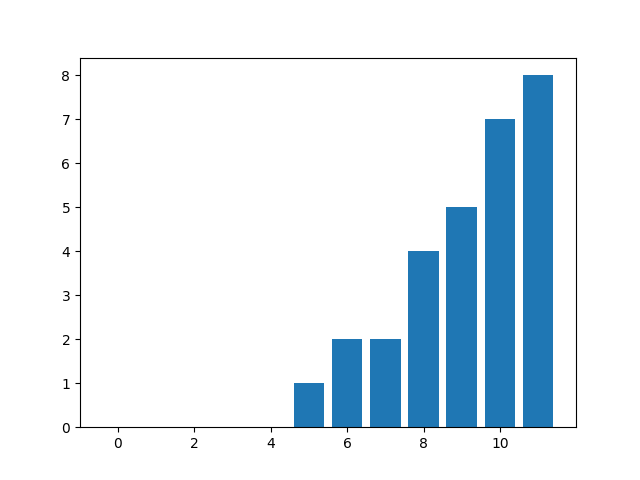
\includegraphics{ps0_template/p1f.png}
    \end{figure} 
\end{itemize}

\section{Basic Image Manipulations (40 points)}	
Do the following by filling out p2.py:
\begin{itemize}

	\item[(c)]
	Add the images together and re-normalize them to have minimum value 0
	and maximum value 1. \textbf{Save and include this image in your report.}
	\begin{figure}[H]
    \vspace{-0.4cm}
    \begin{center}
        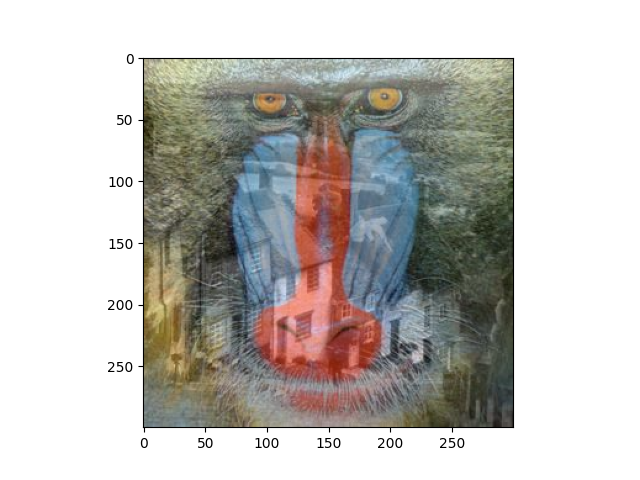
\includegraphics[height=10cm]{ps0_template/p2c.png}
    \end{center}
    \vspace{-1.1cm}
    \end{figure}
    
	\item[(d)]
	Create a new image such that the left half of the image is the left half of
	image1 and the right half of the image is the right half of image2. \textbf{Save and include this image in your report.}
	\begin{figure}[H]
    \vspace{-0.5cm}
    \begin{center}
    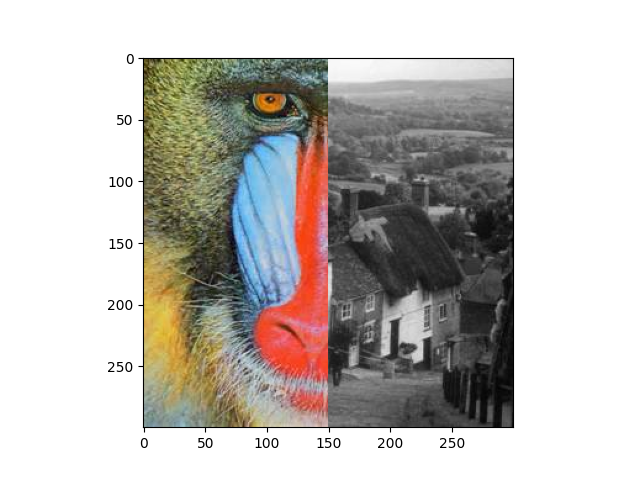
\includegraphics[height=10cm]{ps0_template/p2d.png}
    \end{center}
    \end{figure}
    
	\item[(e)]
	Using a for loop, create a new image such that every odd numbered row is
	the corresponding row from image1 and the every even row is the corresponding row
	from image2 (Hint: Remember that indices start at 0 and not 1 in Python). \textbf{Save and include this image in your report.}
    \begin{figure}[H]
    \vspace{-0.4cm}
    \begin{center}
        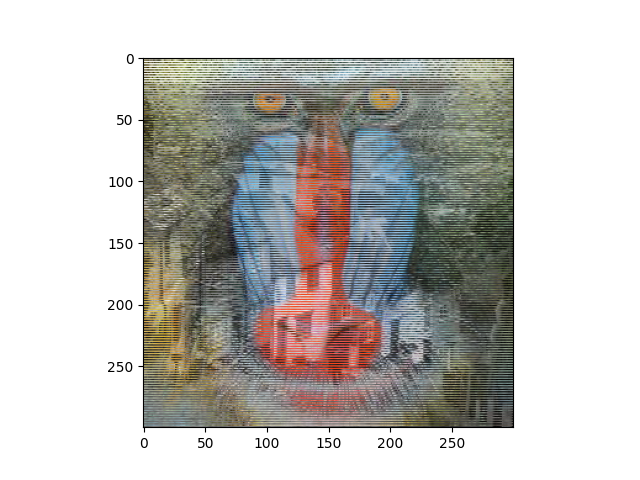
\includegraphics[height=10cm]{ps0_template/p2e.png}
    \end{center}
    \vspace{-1.1cm}
    \end{figure}
	
	\item[(f)]
	Accomplish the same task as part e without using a for-loop (the functions reshape and
  tile may be helpful here). \textbf{Briefly explain the logic of your code in your written report.}
    \begin{figure}[H]
    \vspace{-0.5cm}
    \begin{center}
        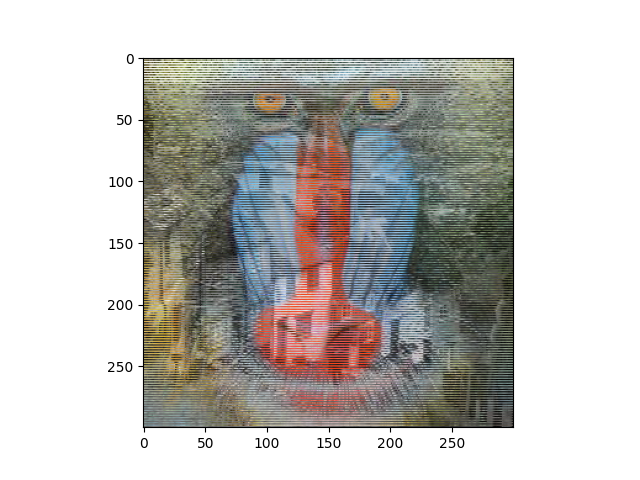
\includegraphics[height=10cm]{ps0_template/p2f.png}
    \end{center}
    \end{figure}

    We can create a mask for each of the image with $0$ at the location where the image doesn't contribute to the final image and $1$ at the location where the image does contribute to the final image. Since, this mask is a repetition of $0$ and $1$, we can use \texttt{np.tile} function. The final image can then be obtained using \texttt{newImage2 = img1*img1\_mask + img2*img2\_mask}.
  
	
	\item[(g)]
	Convert the result from part f to a grayscale image. \textbf{Save and include the grayscale image in your report.}
    \begin{figure}[h]
    \begin{center}
        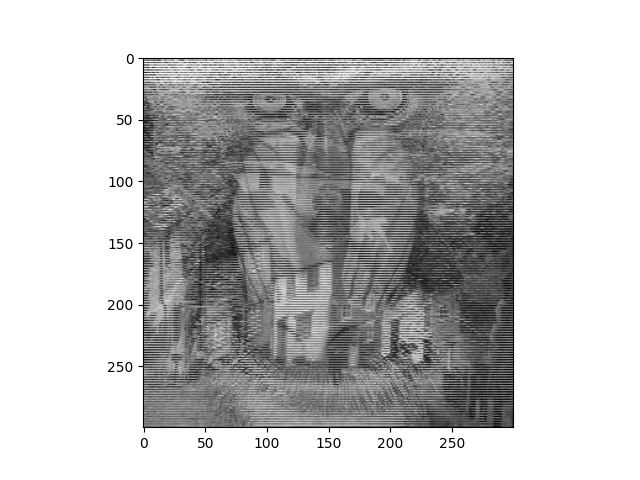
\includegraphics[height=10cm]{ps0_template/p2g.png}
    \end{center}
    \end{figure}
\end{itemize}
	
\section{Singular Value Decomposition (40 points)}
Do the following by filling out p3.py:

\begin{itemize}

	\item[(b)] 
	\textbf{Save and Include the best rank 1 approximation of the (grayscale) image1 in your report.}
    \begin{figure}[H]
    \vspace{-0.5cm}
    \begin{center}
        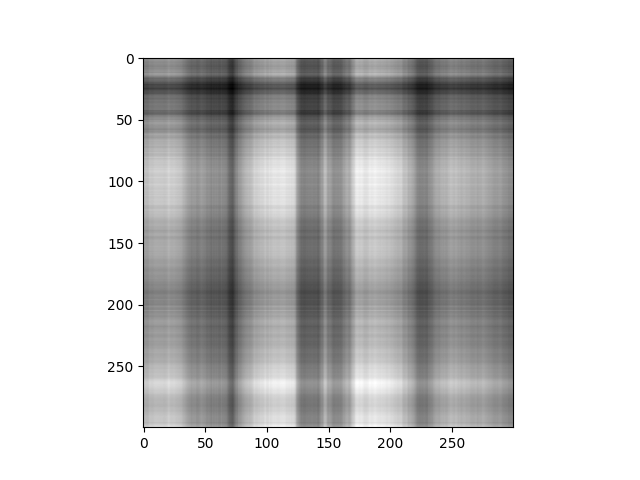
\includegraphics[height=10cm]{ps0_template/p3b.png}
    \end{center}
    \end{figure}

	\item[(c)]
	\textbf{Save and Include the best rank 20 approximation of the (grayscale) image1 in your report.}
    \begin{figure}[H]
    \vspace{-0.5cm}
    \begin{center}
        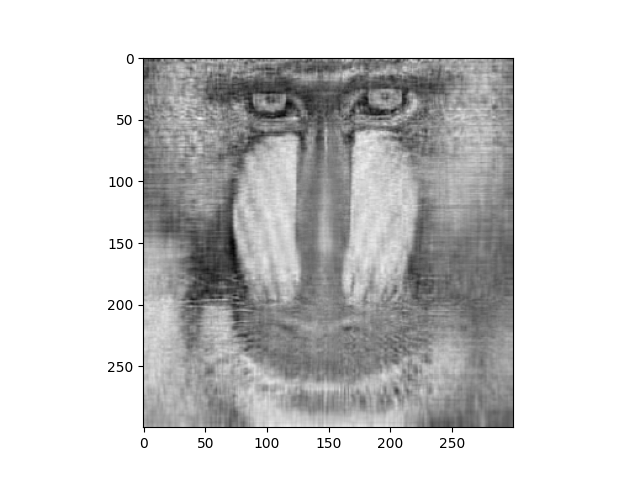
\includegraphics[height=10cm]{ps0_template/p3c.png}
    \end{center}
    \end{figure}
\end{itemize}

\end{document}

